%%%%%%%%%%%%%%%%%%%%%%%%%%%%%%%%%%%%%%%%%
% University/School Laboratory Report
% LaTeX Template
% Version 3.0 (4/2/13)
%
% This template has been downloaded from:
% http://www.LaTeXTemplates.com
%
% Original author:
% Linux and Unix Users Group at Virginia Tech Wiki 
% (https://vtluug.org/wiki/Example_LaTeX_chem_lab_report)
%
% License:
% CC BY-NC-SA 3.0 (http://creativecommons.org/licenses/by-nc-sa/3.0/)
%
%%%%%%%%%%%%%%%%%%%%%%%%%%%%%%%%%%%%%%%%%

%----------------------------------------------------------------------------------------
%	PACKAGES AND DOCUMENT CONFIGURATIONS
%----------------------------------------------------------------------------------------

\documentclass{article}

\usepackage[version=3]{mhchem} % Package for chemical equation typesetting
\usepackage{siunitx} % Provides the \SI{}{} command for typesetting SI units

\usepackage[top=1in, bottom=1in, right=1in, left=1in]{geometry}

%Add code formating
\usepackage{listings}
\lstset{tabsize=2}

\usepackage{hyperref}

\usepackage{amssymb}

\usepackage{enumerate}

\usepackage{multicol} % Multi-column support

%Add extra support for image placement
\usepackage{float}

\usepackage{mcode}

\usepackage{graphicx} % Required for the inclusion of images

\setlength\parindent{0pt} % Removes all indentation from paragraphs

\renewcommand{\labelenumi}{\alph{enumi}.} % Make numbering in the enumerate environment by letter rather than number (e.g. section 6)

%\usepackage{times} % Uncomment to use the Times New Roman font

% Setup how hyperlinks look
\usepackage{xcolor}
\hypersetup{
	colorlinks,
	linkcolor={red!50!black},
	citecolor={blue!50!black},
	urlcolor={blue!80!black},
}

%----------------------------------------------------------------------------------------
%	DOCUMENT INFORMATION
%----------------------------------------------------------------------------------------

\title{Keysight Hacking Platform Hardware Overview} % Title

\author{Blake \textsc{Vermeer}} % Author name

\date{\today} % Date for the report

\begin{document}

\maketitle % Insert the title, author and date

\begin{center}
\begin{tabular}{l r}
Date Performed: & March 26, 2017 \\ % Date the experiment was performed
Company: & Keysight Technologies % Company
\end{tabular}
\end{center}

% If you wish to include an abstract, uncomment the lines below
% \begin{abstract}
% Abstract text
% \end{abstract}

%----------------------------------------------------------------------------------------
%	OVERVIEW
%----------------------------------------------------------------------------------------
\section{Overview}

This document gives a general hardware architecture overview of the Keysight Hacking Platform (KHP), a general hardware overview of the Raspberry Pi 3 and a detailed description of how the touch-screen is connected to the Raspberry Pi 3.


%----------------------------------------------------------------------------------------
%	RPi 3 Block Diagram
%----------------------------------------------------------------------------------------
\section{Raspberry Pi 3 Block Diagram}

At the heart of the Keysight Hacking Platform is a Raspberry Pi 3. The Raspberry Pi 3 is a general purpose embedded ARM Linux device. 

	\begin{minipage}{0.5\textwidth}
		
		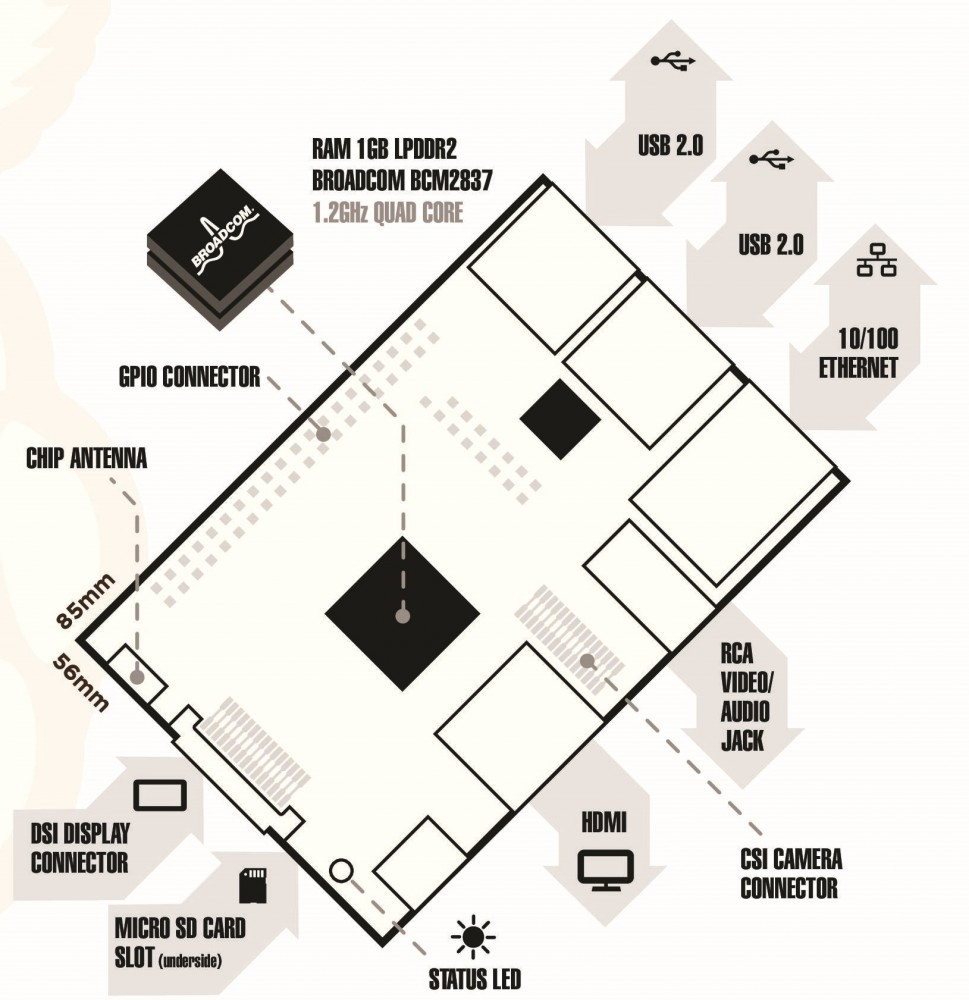
\includegraphics[width=0.95\textwidth]{pics/Raspberry-Pi-3_Block_Diagram.jpg}
		
		%\begin{figure}[H]
		%	\centering
		%	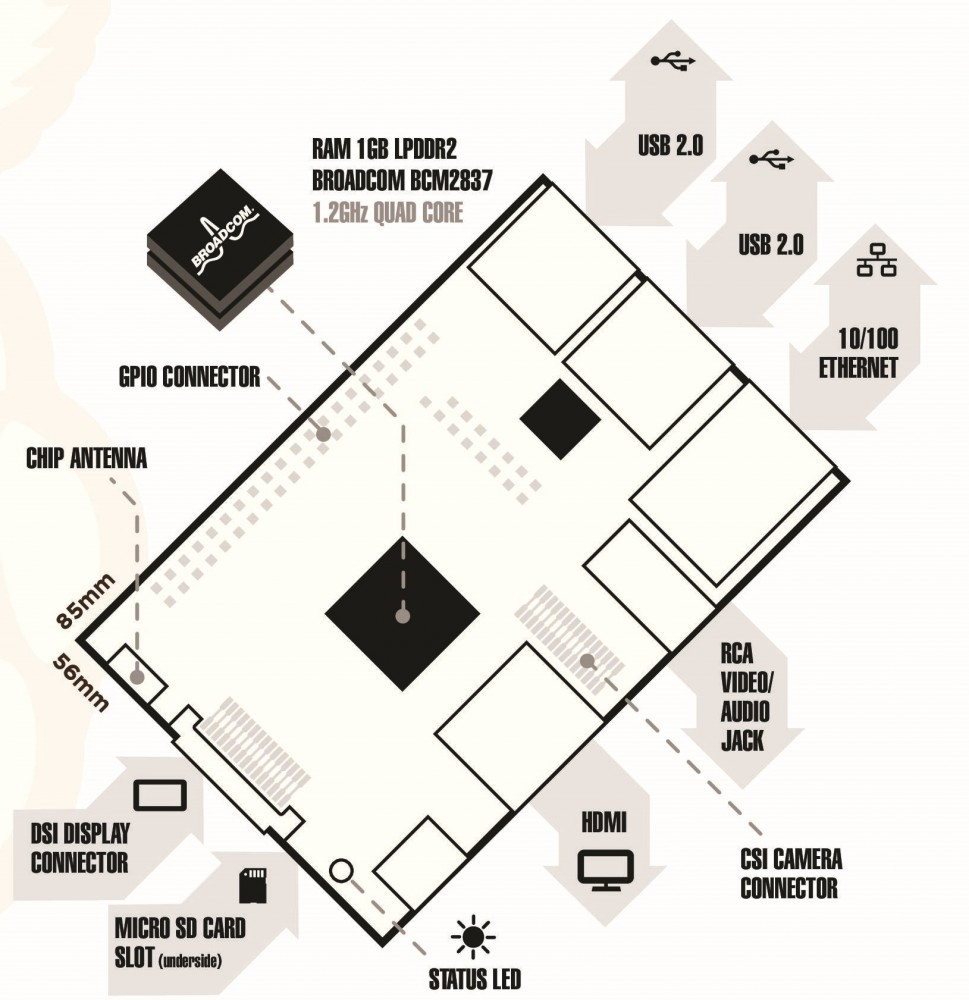
\includegraphics[scale=0.3]{pics/Raspberry-Pi-3_Block_Diagram.jpg}
		%	\caption{Raspberry Pi 3 Block Diagram}
		%	\label{RPi_3_Block_Diagram}
		%\end{figure} 
	
	\end{minipage}
	\begin{minipage}{0.45\textwidth}
		
		\begin{itemize}
			\item CPU: 1.2 GHz quad-core ARM Cortex A53
			\item Memory: 1 GB LPDDR2-900 SDRAM
			\item 4 USB ports (Max current draw of 1.2A combined on all the USB ports)
			\item 10/100 Ethernet
			\item HDMI
			\item Bluetooth 4.0
			\item 802.11n Wireless LAN
			\item Combination RCA Video / Audio jack
			\item 40 Pin GPIO Connector
		\end{itemize}
	
	\end{minipage}








%----------------------------------------------------------------------------------------
%	RPi 3 GPIO Usage Overview
%----------------------------------------------------------------------------------------
\section{Raspberry Pi 3 Used GPIO Lines}

This section explains which GPIO lines are used by the touchscreen and which GPIO lines are connected to the four push-buttons. The LCD is driven by a Serial Peripheral Interface (SPI) bus. The Raspberry Pi 3 contains three independent SPI bus drivers and in the case the screen is connected to SPI bus 0. The Raspberry Pi 3 has two I2C buses available on the GPIO header and both are used by the screen (I2C bus 0 is used by the configuration EEPROM and I2C bus 1 is used by the touchscreen). Figure \ref{Screen_Used_GPIO} shows the GPIO lines used by the touchscreen and the LCD.

	\begin{figure}[H]
		\centering
		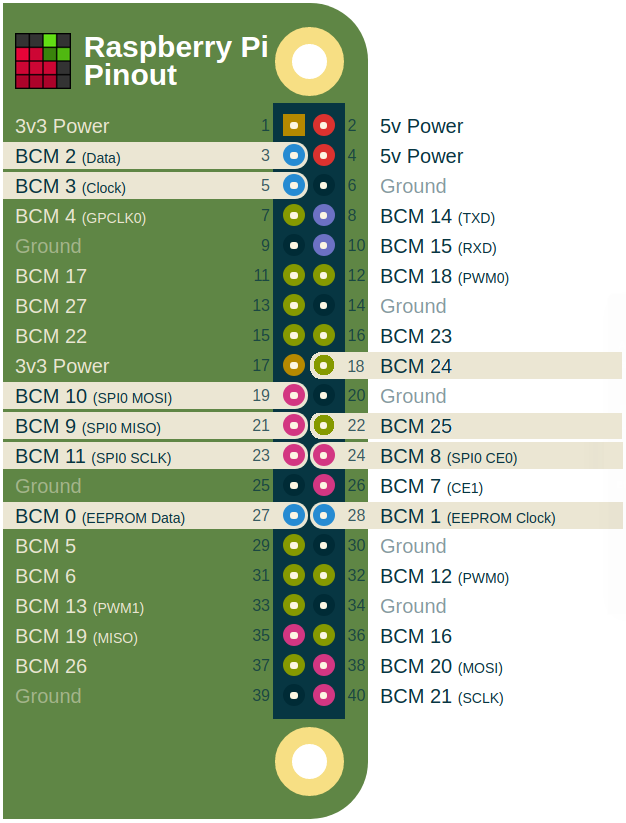
\includegraphics[scale=0.3]{pics/GPIO_Used_By_Screen.png}
		\caption{GPIO Lines Used by the Screen}
		\label{Screen_Used_GPIO}
	\end{figure} 

	\begin{table}[H]
		\centering
		
		\begin{tabular}[H]{| c | c |}
			\hline
			\textbf{Communication Bus} & \textbf{Used by} \\
			\hline
			I2C Bus 0 & Configuration EEPROM \\
			\hline
			I2C Bus 1 & Touchscreen \\
			\hline
			SPI Bus 0 & LCD \\
			\hline
			SPI Bus 1 & nothing \\
			\hline
		\end{tabular}
	\end{table}


The touch-screen also features four hardware push-buttons which are connected directly to GPIO lines as shown in the section of the touch-screen schematic shown in Figure \ref{Push_buttons_schematic}.


	\begin{figure}[H]
		\centering
		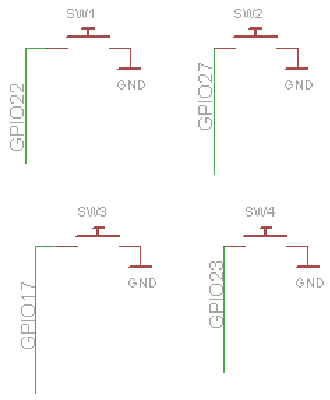
\includegraphics[width=0.25\textwidth]{pics/PiTFT_2-8_push-buttons_section_schematic.png}
		\caption{Screen Push-Buttons Schematic}
		\label{Push_buttons_schematic}
	\end{figure}


In order to use the push-buttons, the GPIO lines connected to the push-buttons need to be configured as inputs and the internal pull-up resistors enabled (external pull-up resistors could alternatively be used). The push-buttons are connected to the GPIO lines on the Raspberry Pi 3 header as shown in Figure \ref{Push_buttons_GPIO}.


	\begin{figure}[H]
		\centering
		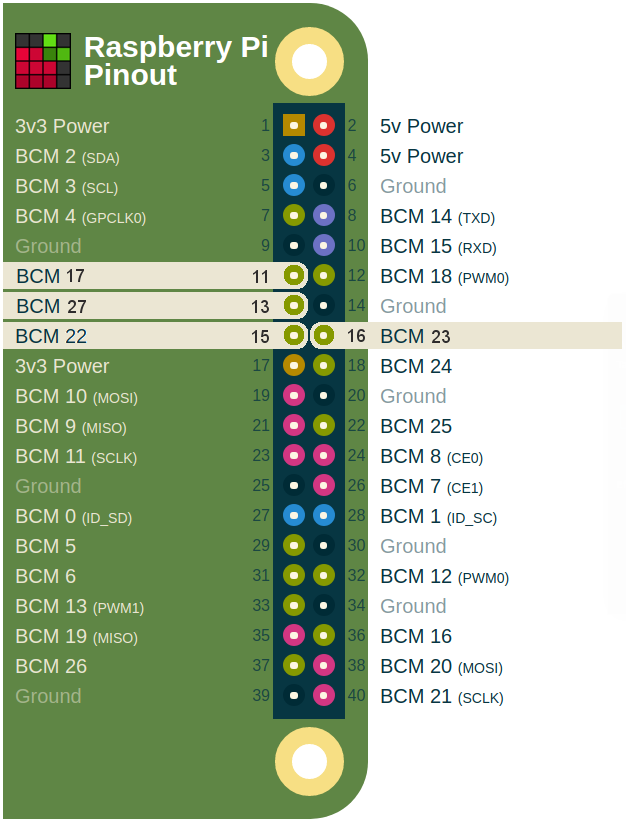
\includegraphics[scale=0.3]{pics/PiTFT_2-8_Switches_GPIO.png}
		\caption{GPIO Lines used by Push-Buttons}
		\label{Push_buttons_GPIO}
	\end{figure}


It is also possible to figure out which push-button is connected to which GPIO line by looking at the silkscreen labels next to the push-buttons on the screen. Note: the numbers on the labels are the Broadcom pin numbers (BCM numbers) and not the physical pin numbers!



	\begin{figure}[H]
		\centering
		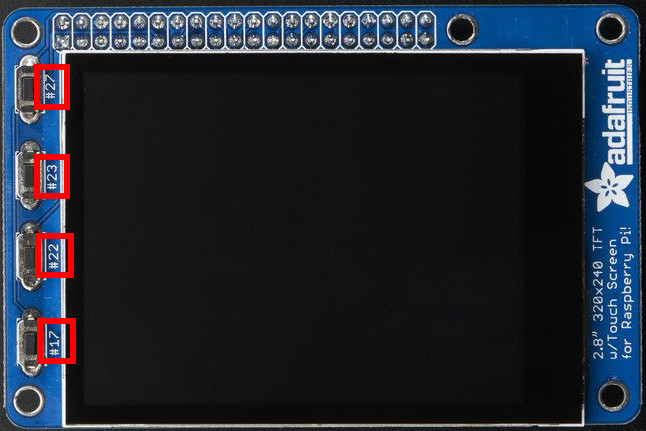
\includegraphics[width=0.65\textwidth]{pics/PiTFT_Plus_2_8_Overhead.jpg}
		\caption{Push Button Labels}
		\label{Push_Button_Labels}
	\end{figure}


In summary, Figure \ref{All_Used_GPIO} shows all the GPIO lines in use.


	\begin{figure}[H]
		\centering
		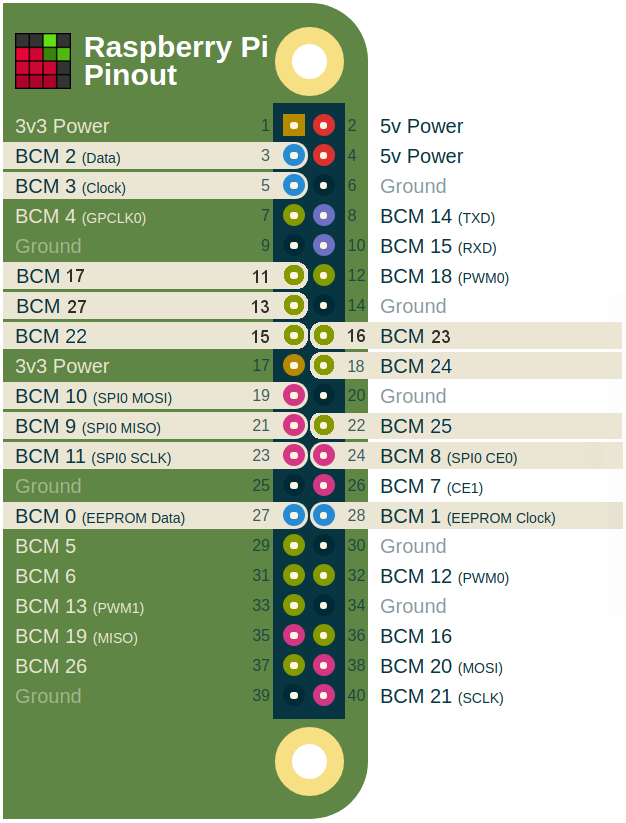
\includegraphics[scale=0.3]{pics/All_Used_GPIO.png}
		\caption{All Used GPIO}
		\label{All_Used_GPIO}
	\end{figure}

%----------------------------------------------------------------------------------------
%	RPi 3 Available GPIO and Interfaces
%----------------------------------------------------------------------------------------
\section{Raspberry Pi 3 Available GPIO and Interfaces}

After accounting for the pins used by the LCD screen, touchscreen, and hardware buttons there are 13 GPIO lines left unused (17 it you don't need to use the HW buttons). These unused GPIO lines can be used as general input pins or outputs (hence the name GPIO - General Purpose Input Output). To use the extra GPIO lines, the wiringPi library can be used or the \textbf{tiny\_gpio} class in the \textbf{hw\_button\_example} program. \\

Also, SPI bus 1 is unused and can be used to communicate with external SPI devices such as the MCP3008 ADC. For more information on how to use the MCP3008 ADC refer to the \textbf{Using\_the\_MCP3008\_ADC} document. \\

	\begin{figure}[H]
		\centering
		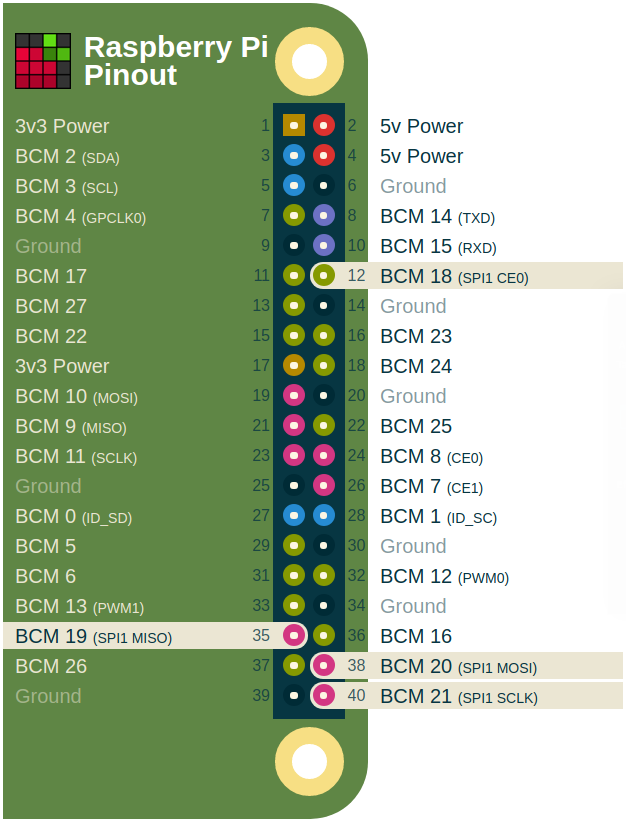
\includegraphics[width=0.5\textwidth]{pics/SPI_Bus1_CS0.png}
		\caption{Raspberry Pi 3, SPI Bus 1}
		\label{SPI_Bus1}
	\end{figure}

It should be noted that all the GPIO lines on the Raspberry Pi 3 are 3.3V lines and are \textcolor{red}{\textbf{NOT}} 5V tolerant!


%----------------------------------------------------------------------------------------
%	APPENDIX
%----------------------------------------------------------------------------------------

%\newpage
%\section{Appendix}

%\begin{enumerate}

	
%	\item[1. a.)] \lstinputlisting{../MATLAB/problem_1a.m}
	

%\end{enumerate}






%----------------------------------------------------------------------------------------


\end{document}